\documentclass[10pt]{article}
\usepackage[margin=0.8in]{geometry}
\usepackage{graphicx}
\usepackage{booktabs}
\title{Supplementary Material: Reliable Strictly Local Floorplan Editing}
\author{Anonymous Submission}
\date{}
\begin{document}
\maketitle

\section{Protocol Boundaries}
Oracle-control rows are capacity evidence and are not deployable. Predicted
controls are target-free at inference. Aligned, canonical-instance, and typed
graph metrics are separate protocols. Raw fpeval watertightness is always
reported independently of functional and componentwise diagnostics.

\section{Operation-Success Predicates}
Room type and addition require the requested target class to dominate changed
pixels. Room removal requires source-class removal or merging. Object deletion
requires removal of the requested family. The old control source is an allowed
editing input; source drift is reported separately from locality violations.

\section{Reviewer-Facing Evidence}
The main paper reports positive oracle evidence and retained predicted-control
limitations. The development test exposure is not presented as held-out
evidence. A fresh held-out run is required after the model and thresholds are
frozen.

\begin{figure*}[t]
\centering
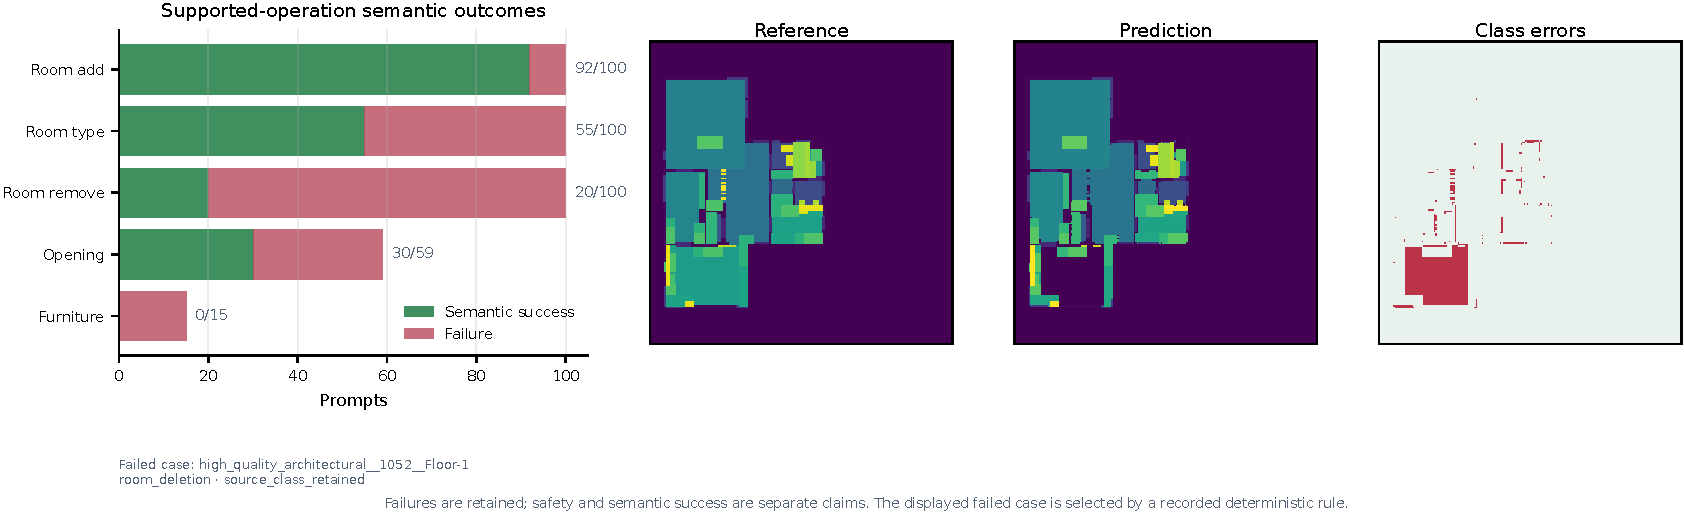
\includegraphics[width=\textwidth]{figures/floorplan_failure_taxonomy_v1.pdf}
\caption{Semantic outcomes for supported operations with the actual prompt
denominator. Failures are retained and are not reclassified as abstentions.}
\label{fig:failures}
\end{figure*}

\end{document}
